%%%%%%%%%%%%%%%%%%%%%%%%%%%%%%%%%%%%%%%%%
% Short Sectioned Assignment
% LaTeX Template
% Version 1.0 (5/5/12)
%
% This template has been downloaded from:
% http://www.LaTeXTemplates.com
%
% Original author:
% Frits Wenneker (http://www.howtotex.com)
%
% License:
% CC BY-NC-SA 3.0 (http://creativecommons.org/licenses/by-nc-sa/3.0/)
%
%%%%%%%%%%%%%%%%%%%%%%%%%%%%%%%%%%%%%%%%%

%----------------------------------------------------------------------------------------
%	PACKAGES AND OTHER DOCUMENT CONFIGURATIONS
%----------------------------------------------------------------------------------------

\documentclass[paper=a4, fontsize=11pt]{scrartcl} % A4 paper and 11pt font size

\usepackage[T1]{fontenc} % Use 8-bit encoding that has 256 glyphs
%\usepackage{fourier} % Use the Adobe Utopia font for the document - comment this line to return to the LaTeX default
\usepackage[english]{babel} % English language/hyphenation
\usepackage{amsmath,amsfonts,amsthm} % Math packages

\usepackage{lipsum} % Used for inserting dummy 'Lorem ipsum' text into the template

\usepackage{graphicx}
\usepackage{caption}
\usepackage{subcaption}

\usepackage{sectsty} % Allows customizing section commands
\allsectionsfont{\centering \normalfont\scshape} % Make all sections centered, the default font and small caps

\usepackage{fancyhdr} % Custom headers and footers
\pagestyle{fancyplain} % Makes all pages in the document conform to the custom headers and footers
\fancyhead{} % No page header - if you want one, create it in the same way as the footers below
\fancyfoot[L]{} % Empty left footer
\fancyfoot[C]{} % Empty center footer
\fancyfoot[R]{\thepage} % Page numbering for right footer
\renewcommand{\headrulewidth}{0pt} % Remove header underlines
\renewcommand{\footrulewidth}{0pt} % Remove footer underlines
\setlength{\headheight}{13.6pt} % Customize the height of the header

\numberwithin{equation}{section} % Number equations within sections (i.e. 1.1, 1.2, 2.1, 2.2 instead of 1, 2, 3, 4)
\numberwithin{figure}{section} % Number figures within sections (i.e. 1.1, 1.2, 2.1, 2.2 instead of 1, 2, 3, 4)
\numberwithin{table}{section} % Number tables within sections (i.e. 1.1, 1.2, 2.1, 2.2 instead of 1, 2, 3, 4)

\setlength\parindent{0pt} % Removes all indentation from paragraphs - comment this line for an assignment with lots of text

%----------------------------------------------------------------------------------------
%	TITLE SECTION
%----------------------------------------------------------------------------------------

\newcommand{\horrule}[1]{\rule{\linewidth}{#1}} % Create horizontal rule command with 1 argument of height

\title{	
\normalfont \normalsize 
\textsc{ETH Zurich, D-INFK} \\ [25pt] % Your university, school and/or department name(s)
\horrule{0.5pt} \\[0.4cm] % Thin top horizontal rule
\huge Computer Vision: Exercise 2 \\ % The assignment title
\horrule{2pt} \\[0.5cm] % Thick bottom horizontal rule
}

\author{Igor Pesic} % Your name

\date{\normalsize\today} % Today's date or a custom date

\begin{document}

\maketitle % Print the title


\section{Camera Calibration}

\subsection{Data normalization}
In this part of the code, I have normalized the data as described on the exercise sheet. So the normalized data is shifted around the origin and the average distance to the origin of the shifted data is $\sqrt{2}$ and $\sqrt{3}$ for 2D and 3D point respectively. Transformation matrices $T$ and $U$ are the inverse of the matrices where diagonals are filled with the scales and the last column represents the minus mean point in homogeneous coordinates. 

\subsection{DLT and Gold Standard Algorithm}
I have implemented these two algorithms exactly as described on the exercise sheet, although the matrix $A$ from the equation $AP=0$ is a vertical concatenation of sub-matrices for each data point. Thus the size of matrix $A$ is $2n \times 12$. The selected points are shown in Figure \ref{fig:orig} and their reprojections in Figure \ref{fig:repr}.\\
\\
The reprojection errors are given in the Table \ref{tab:errors} The error is defined as the average euclidean distance to the original point. From the table we can conclude that the normalization has the positive effect on the reprojection error, probably due to stability improvements of the algorithm. Also the Gold Standard Algorithm has improved the results on the normalized data.

\begin{figure}
	\centering
  	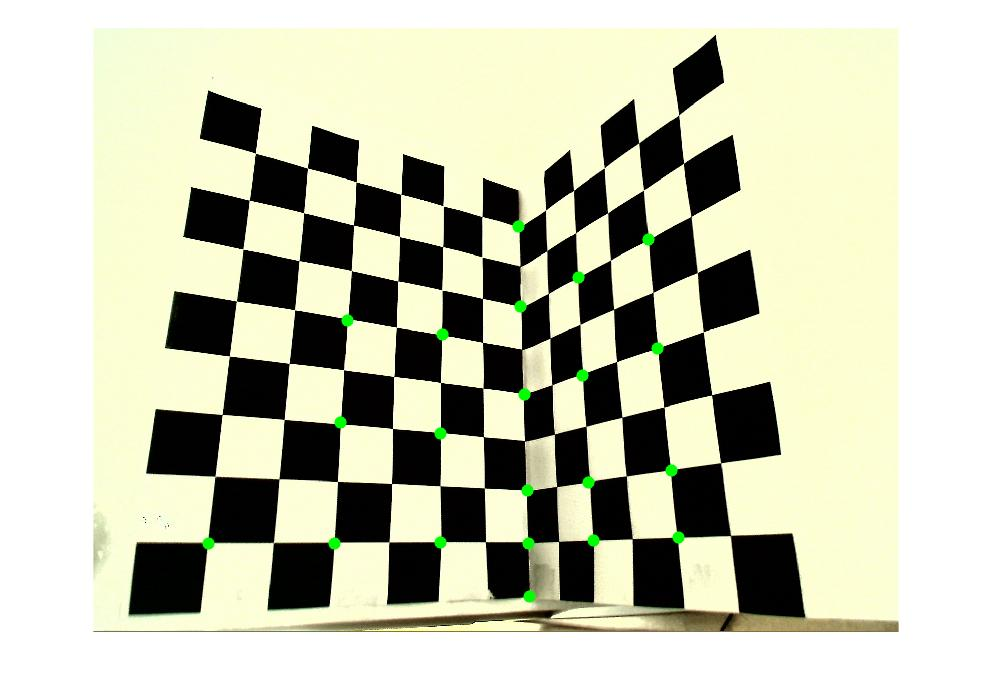
\includegraphics[width=90mm]{data.jpg}
	\caption{Selected points}
	\label{fig:orig}
\end{figure}

\begin{figure}
\centering
\begin{tabular}{cc}
  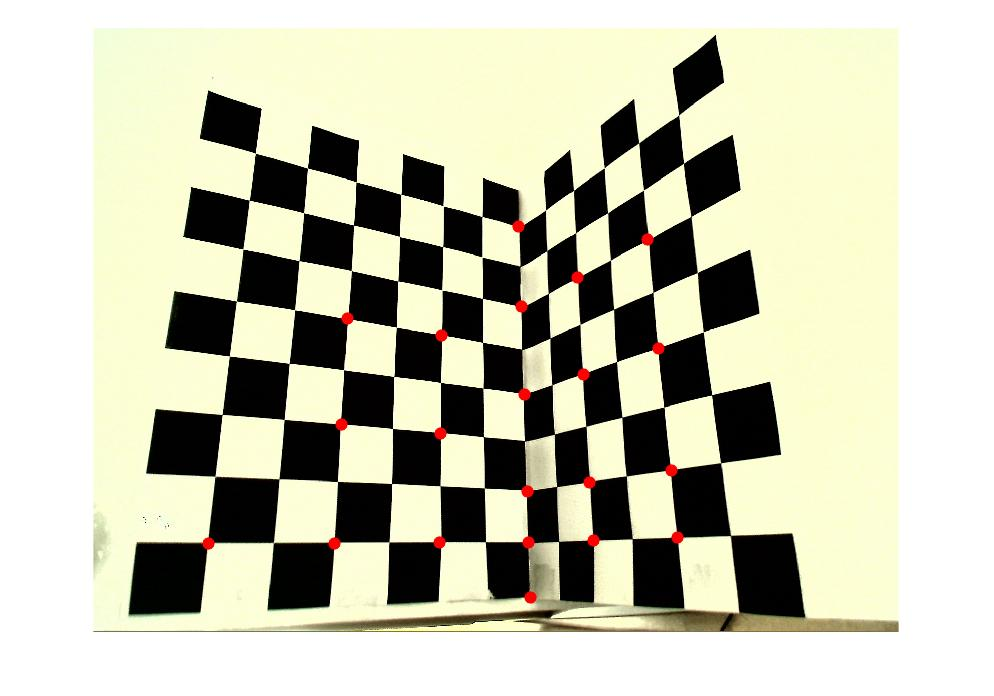
\includegraphics[width=85mm]{dlt_no_norm.jpg} &   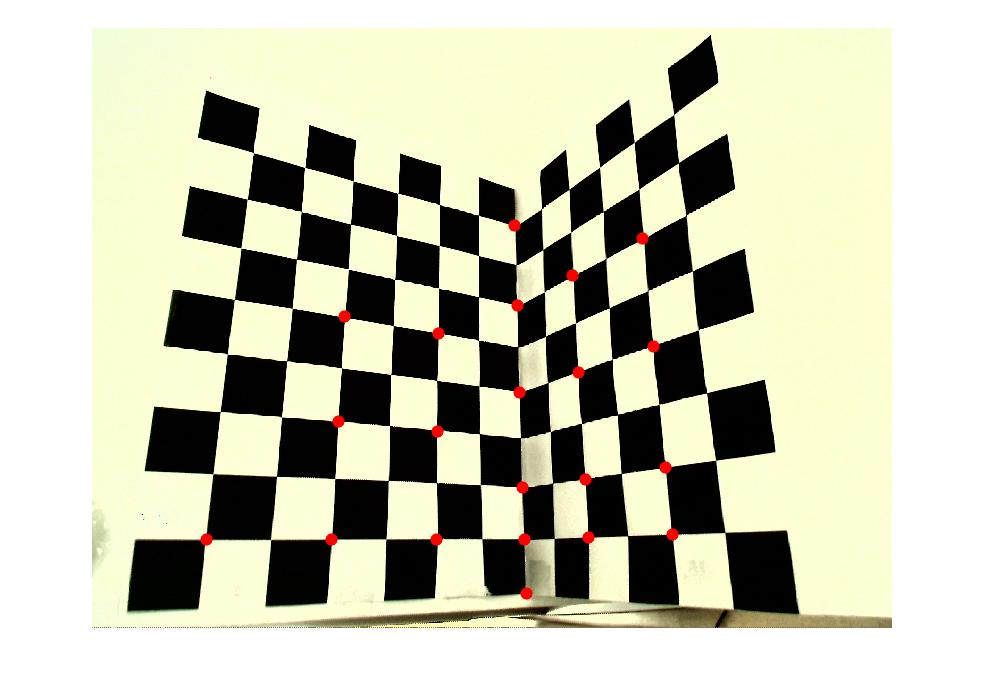
\includegraphics[width=85mm]{dlt.jpg} \\
(a) DLT & (b) DLT with normalization \\[6pt]
  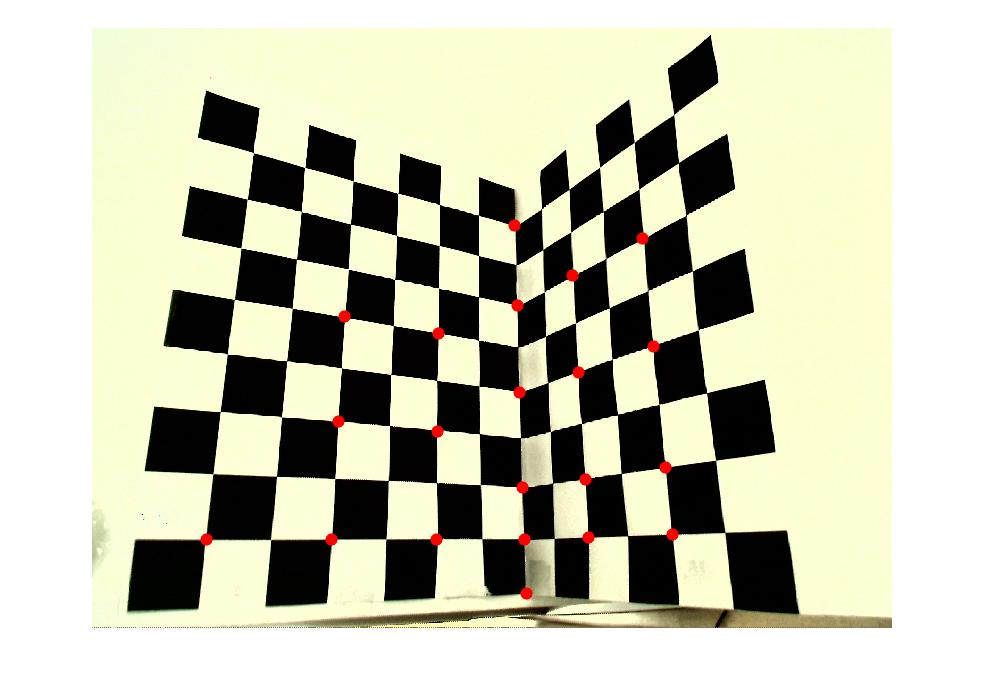
\includegraphics[width=85mm]{gold_no_norm.jpg} &   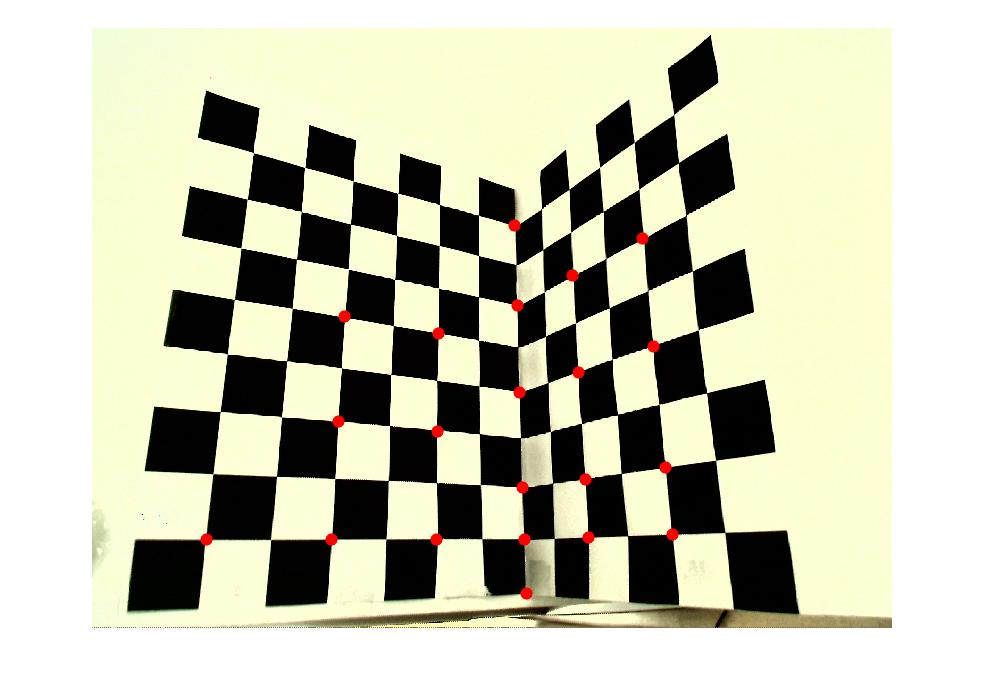
\includegraphics[width=85mm]{gold.jpg} \\
(c) Gold & (d) Gold with normalization \\[6pt]

\end{tabular}
\caption{Reprojected points}
\label{fig:repr}
\end{figure}

\begin{table}[]
\centering
\caption{Reprojection errors}
\label{tab:errors}
\begin{tabular}{|l|l|l|}
\hline
 & Without Normalization & With Normalization \\ \hline
DLT   & 1.6144                & 1.6129             \\ \hline
Gold  & 1.6144                & 1.6009             \\ \hline
\end{tabular}
\end{table}




\end{document}